
%%%%%%% Probably want this in the simulation section....
%  \subsection{Simulation Setup}
%    All the simulations were run on a custom built workstation with an Intel Xeon CPU E5-2650 (1.2 GHz, 20 MB cache size) and 32 GB RAM under Red Hat Enterprise Linux Server release 6.5 (Santiago). 
%    Running the simulations with OpenMP, took advantage of the 16 processers of the Intel Xeon CPU, each with 2 threads. 
%    The GNU fortran compiler version 4.4.7 was used for the typical simulation results; compiler arguments were \begin{verbatim} -O3 -fdefault-real-8 -fopenmp .\end{verbatim}
%    The Intel Fortran compiler version 14.0.2 was used for the speed results; compiler arguments were \begin{verbatim} -O3 -r8 -openmp. \end{verbatim}
%
%    The simulations were solved on a $1024 \times 1024$ grid, using $\Delta t = 10^{-2}$.
%     
%     % If it's completed and works, talk about the openACC use here.
  
\section{Method Comparisons}
%This section needs a complete re-write

The main idea to be told in this section is an explaintation and the results for the numerous tests on the methods.
A number of tests can be done, both for the main purpose of comparing semi- and fully-implicit methods and also to just verify the method works.
This means that the first test should include the convergence test, both for grid size and delta t.
Something like:
\subsection{Grid Size Convergence}
  To observe the validity of the method, a test on the convergence of solutions based on the scrutiny of the spatial discritization is done.

  % The idea with these is to have the different methods all converge, not neccessarily 
  % at the same pSize value, but just enought that it is resonbable. A plosible 
  % item to try is either useing the 1D problem travelling wave example, or instead 
  % use the 2d example with the epsilon value that is compared between two adjacent
  % pSize values (it'd be like what was done for the Scientific computing course.
  \begin{figure}
    \centering
    \begin{tabular}{c c}
%    \includegraphics{converge_spatial_a.eps} &
%    \includegraphics{converge_spatial_b.eps} \\
    (a) & (b) \\
%    \includegraphics{converge_spatial_c.eps} &
%    \includegraphics{converge_spatial_d.eps} \\
    (c) & (d) 
    \end{tabular}
    \caption{A series of plots show the convergence of solutions based on changes in $\Delta x$ using $eSoln = 10^n$ for (a) $n = -1$, (b) $n = -4$, (c) $n = -8$, and (d) $n = -12$.} 
    \label{fig:converge_spatial}
  \end{figure}

\subsection{$\Delta t$ Convergence}
  Same idea here as was done in the grid size section. This should show that theere exist a resonable rselection for $\Delta t$ that results in a relativly aaccurate solution for each choice in $eSoln$.

  \begin{figure}
    \centering
    \begin{tabular}{c c}
%    \includegraphics{converge_temporal_a.eps} &
%    \includegraphics{converge_temporal_a.eps} \\
    (a) & (b) \\
%    \includegraphics{converge_temporal_a.eps} &
%    \includegraphics{converge_temporal_a.eps} \\
    (c) & (d)
    \end{tabular}
    \caption{A series of plots showing the convergece of solutions based on changes in $\Delta t$ using $eSoln = 10^n$ for (a) $n = -1$, (b) $n = -4$, (c) $n = -8$, and (d) $n = -12$.} 

  \end{figure}
   
\subsection{Error Computations}
This is going to be a whole section dedicated to the description of my error calculation. Things to include here:
\begin{itemize}
  \item Why I need this?
  \item How do I compute it?
  \item What exactly did I compute?
  \item What program did I use? (R probably....)
  \item Maybe run though a trivial Fisher equation problem to confirm that it works ?
  \item Should try to show that a number of error computations will be used.
    \begin{itemize}
      \item $\epsilon_{sol}$

      \item Use $\epsilon_{sol}$ with Absolute-value norm (just compare values)
      \item Use $\epsilon_{sol}$ with L2-norm (euclidean norm), which I'm not really sure how to apply....
      \item Use $\epsilon_{sol}$ with Linf-norm, (max norm), which is just comparing the maximum of each solution?
      \item What is currently known as $\delta_k$ (Definetly re-name this later)
    \end{itemize}
\end{itemize}

  % Also mention the Accuracy of the solutions by using the norm of each solution compared to the  most accurate one.... (Maybe take a solution at a higher grid resolution?, not sure what to do here)
  A comparison between the semi-implicit and fully-implicit method can be accomplished by looking at both their computation time and the accuracy of the solution.
  The computation time is computed by the system clock from the start of the algorithm to the end of the algorithm. 
  The accuracy of the solution can be found by computing the normed-difference between two solutions, as follows,
  \begin{equation}
    \epsilon_{sol} = {||u_1 - u_2||}
  \end{equation}
  where $u_1, u_2$ are the point wise value of $\mathcal{M}$, for two different solutions.
  This is not a relative error because of the large number of zero valued points. 
  The two solutions here are with the solution at the current grid size and the solution at the next smallest grid size.
  This is because, the samller the grid refinement, the more accurate the solution. 
  Thus to compare the accuracy of methods, this will be used.

  The accuracy of this method depends on the grid size used. A convergence analysis is done to observe at what resolution sufficient accuracy is seen. This is done by comparing the relative error in average $M$ between two solutions with different $\Delta x$. We call this difference $\delta$, which we compute as
  \begin{equation} \label{equ:converg_delta}
      \delta_k = \frac{\left|\overline{M}_{k+1} - \overline{M}_{k} \right|}{\overline{M}_{k+1}}
  \end{equation}
  where $\overline{M}_{k}(t)$ is the average biomass at time $t$, solved with $\Delta x = 2^{-k}$. Figure \ref{fig:converg_average} was computed using (\ref{equ:converg_delta}) with $k = 7,8,...,14$. 
  
  
  \begin{figure}[!htb]
    \centering
%          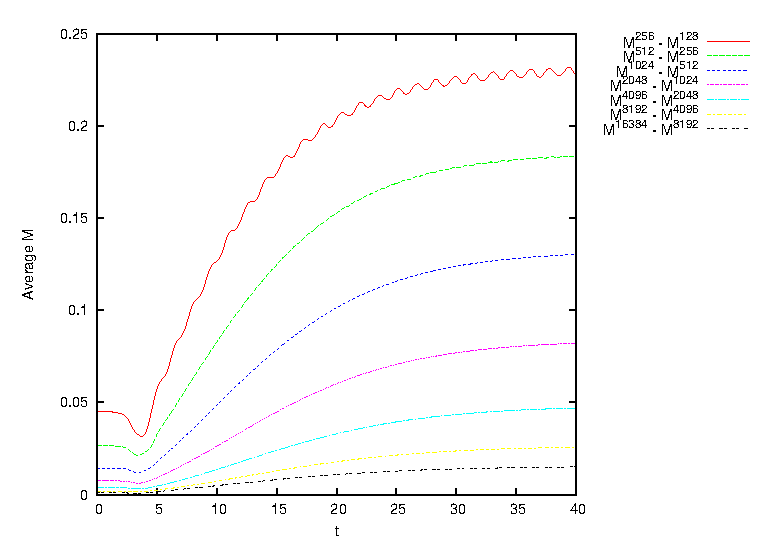
\includegraphics[scale=0.7]{converg_total.eps}
          \caption{Comparison of mean $M$, using (\ref{equ:converg_delta}) with $i = 7,8,...,14$}
          \label{fig:converg_average}
  \end{figure}
  
  This convergence analysis shows a relative error less then $0.02\%$ can be achieved by using $\Delta x = 2^{-13}$. This is considered an sufficient accuracy.
  %!%
  %!%
  %!% FIND A SOURCE THAT SAYS THIS IS ACCURATE ENOUGH
  %!%
  %!%
  
  A second convergence result can be done by instead comparing each gridpoint between solutions. If we define 
  \begin{equation} \label{equ:converg_sigma}
      \sigma_k(t) = 2^{-k} \sum_{i,j} |M^{k+1}(t, x_i, y_j) - M^k(t, x_i, y_i)|,
  \end{equation}
  and 
  \begin{equation} \label{equ:converg_rho}
      \rho_k = \frac{1}{n(T)} \sum_{\forall t \in T} \sigma_k(t).
  \end{equation}
  In (\ref{equ:converg_sigma}), $M^{k}(t,x_i,y_i)$ refers to the biomass when solved with $\Delta x = 2^{-k}$ at time t and gridpoint $(x_i, y_i)$. The value of $\sigma_k(t)$ is the average difference between related gridpoints of solutions solved with different $\Delta x$ values at a specific time $t$. In (\ref{equ:converg_rho}), $n(T)$ refers to the cardinality of $T$, which is the number of outputted times we have. The value of $\rho$ is the average difference across all $t \in T$. 
  %!% Reference the nonexistance figure here.
  
  \begin{figure}[!htb]
    \centering
    %!% Make this figure exist      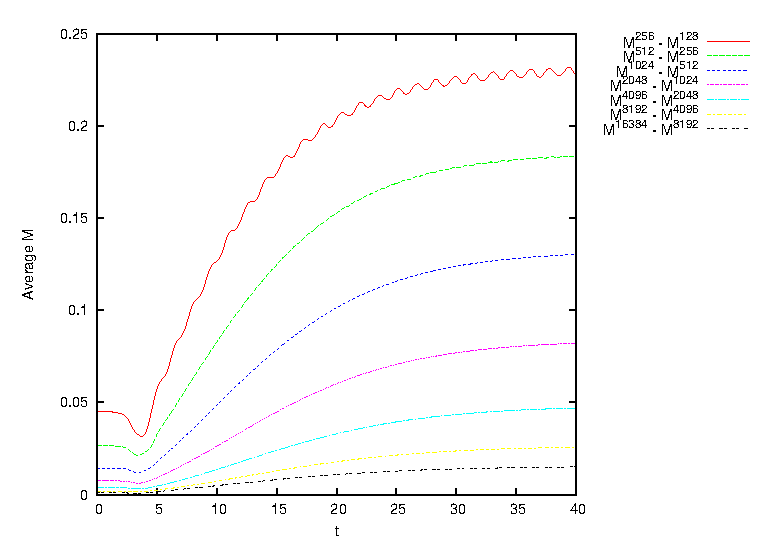
\includegraphics[scale=0.7]{converg_total.eps}
          \caption{Graph of $\rho_k$, for $k = 7,8,...,13$ and $T = 0,2,...,40$}
          \label{fig:converg_rho}
  \end{figure}
  
  This can be extended to check convergence in $\Delta t$ by defining
  \begin{equation} \label{equ:converg_rhoBar}
      \overline{\rho}_{\tau} = \sum_k \rho^{\tau}_k
  \end{equation}
  where $\rho^{\tau}_k$ is the same computations for (\ref{equ:converg_rho}) done with $\Delta t = \tau$.
  
  %!% Add a table of values for \rho^{\tau}
  

\subsection{Results}
  This will be the section that holds the main results for the method comparisons.
  The other comparison will be with where the method is spending its time.
  The fully-implicit method should have less iterations of the linear solver.
  Thus with will be measured as $Iteration 2$. 
  $Iterations 1$ is the number of iterations between solving $M$ and $C$, according to Algorithm \ref{alg:iterateCM}.
  
  The results of the method comparison can be seen in Tabel \ref{tab:tolerance_comparison}.
  
  \begin{table}[h!tb]
    \centering
    \begin{tabular}{|c|c|c|c|c|c|c|}
      \hline
      Tol. 1 & Computation Time & $\epsilon_{sol}$ & Avg. Iter. 1 & Max Iter. 1 & Avg. Iter. 2 & Max Iter. 2 \\
      \hline
      $10^{0}$ & 60.05 & 0.0018 & 1 & 1 & 97.50 & 763 \\
      $10^{-4}$ & 97.72  & 0.0014 & 1.99 & 2 & 86.45 & 1059 \\
      $10^{-8}$ & 117.46 & 0.0013 & 2.92 & 3& 68.67 & 1012 \\
      $10^{-12}$& 126.44 & 0.0011& 3.88 & 5 & 51.84 & 1022 \\
      \hline
    \end{tabular}
    \caption{Results from running simulation with different Tolerance 1 values. Note, Tolerance 1 of $10^{0}$ is the semi-implicit method.}
    \label{tab:tolerance_comparison}
  \end{table}
  
  
  %If I ever get around to it, refere to the results of convergence testing though Python is.
  

